%================================================================
% Beamer presentation for the master's thesis
% "Napovedovanje trkov med vlaki in predori"
% Author: Matic Stare
%================================================================
\documentclass[11pt,aspectratio=169]{beamer}

\usepackage[slovene]{babel}
\usepackage[utf8]{inputenc}
\usepackage[T1]{fontenc}
\usepackage{lmodern}
\usepackage{graphicx}
\usepackage{amsmath,amssymb}
\usepackage{booktabs}
\usepackage{multirow}
\usepackage{algorithm}
\usepackage{algorithmic}
\usepackage{hyperref}

\floatname{algorithm}{Algoritem}

\graphicspath{{../thesis/figures/}}

\usetheme{Madrid}
\usecolortheme{default}
\setbeamertemplate{navigation symbols}{}
\setbeamertemplate{caption}{\raggedright\insertcaption\par}
\setbeamerfont{footnote}{size=\tiny}

\title{Napovedovanje trkov med vlaki in predori}
\subtitle{Magistrsko delo}
\author[M.\ Stare]{Matic Stare \texorpdfstring{\\}{} \small Mentor: doc.\ dr.\ Uroš Čibej}
\institute[FRI UL]{Univerza v Ljubljani \\ Fakulteta za računalništvo in informatiko}
\date{Ljubljana, 2026}

\begin{document}

%----------------------------------------------------------------
% 1. Naslovnica
%----------------------------------------------------------------
\begin{frame}
    \titlepage
\end{frame}

%================================================================
\section{Uvod}
%================================================================

%----------------------------------------------------------------
% 2. Opis problema
%----------------------------------------------------------------
\begin{frame}{Opis problema}
    \begin{columns}[T]
        \begin{column}{0.55\textwidth}
            \begin{itemize}
                \item Statični prerez: obstoječa metoda SŽ; deluje na ravnih predorih.
                \item Težava v ovinkih:
                    \begin{itemize}
                        \item srednji del vagona bližje steni kot sprednji/zadnji,
                        \item vzrok: medosna razdalja.
                    \end{itemize}
                \item Statični prerez tega ne zajame $\rightarrow$ navidez varne razmere $\rightarrow$ trk.
                \item Stopnjuje se z dolžino vagona in ostrostjo ovinka.
            \end{itemize}
        \end{column}
        \begin{column}{0.45\textwidth}
            \centering
            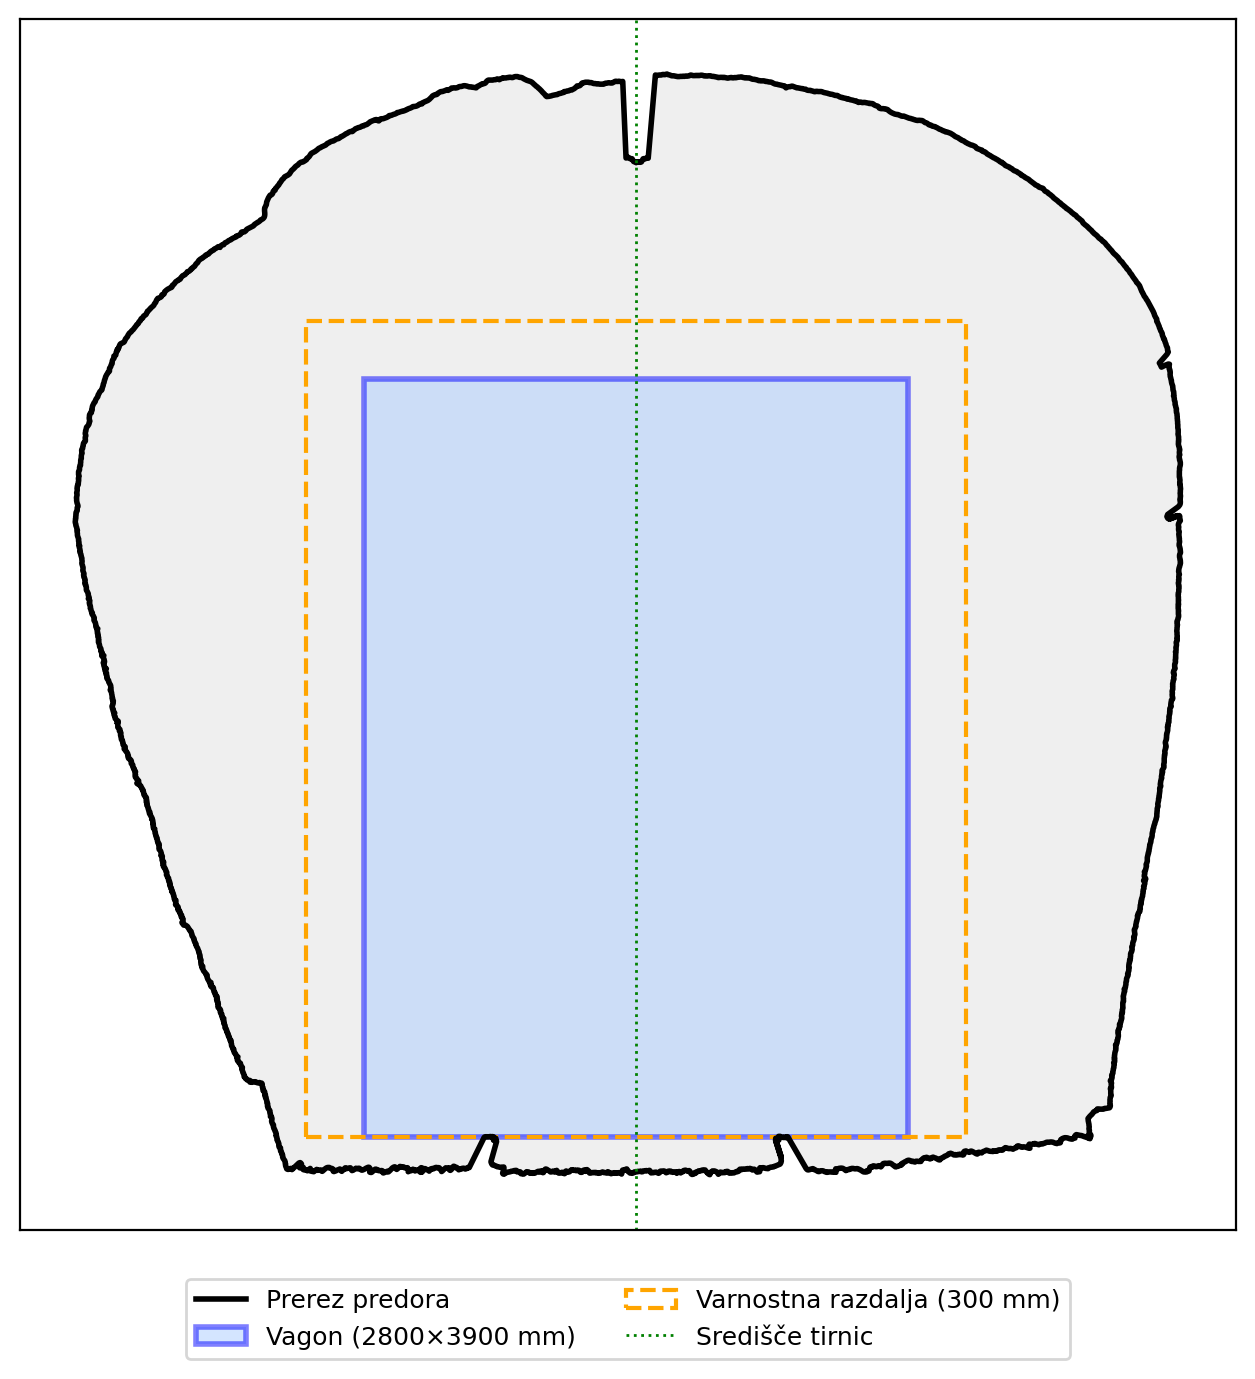
\includegraphics[height=4.5cm]{cross_section.png}\\
            {\scriptsize Statični prerez predora z vlakom.}
        \end{column}
    \end{columns}
\end{frame}

%----------------------------------------------------------------
% 3. Cilj in prispevki
%----------------------------------------------------------------
\begin{frame}{Cilj in prispevki}
    \textbf{Cilj}: dinamično zaznavanje trkov.

    \vspace{0.5em}
    \textbf{Pristop}: obdelava oblaka točk predora $+$ simulacija gibanja vagona.

    \vspace{0.5em}
    \textbf{Prispevki:}
    \begin{itemize}
        \item detektor trkov: geometrija predora + dejansko gibanje vagona;
        \item brušenje vagona: izpeljava največjega varnega modela za dani predor;
        \item prileganje tovora poljubnih oblik;
        \item interaktivna 3D vizualizacija; aplikacija za SŽ.
    \end{itemize}
\end{frame}

%================================================================
\section{Teoretične osnove}
%================================================================

%----------------------------------------------------------------
% 4. Geometrijska predstavitev predora
%----------------------------------------------------------------
\begin{frame}{Geometrijska predstavitev predora}
    \begin{itemize}
        \item Vhod: 2D prerezi pravokotno na os (razmik 0,5 m, 3D laserski skener).
        \item Pretvorba v 3D oblak, ki sledi ukrivljeni poti -- Rodriguesova formula:
    \end{itemize}
    \begin{equation*}
        \boldsymbol{p}'_i = \boldsymbol{R}\,(\boldsymbol{p}_i - \boldsymbol{t}_{\text{center}}), \quad
        \boldsymbol{R} = \boldsymbol{I} + \sin\theta\,\boldsymbol{K} + (1-\cos\theta)\,\boldsymbol{K}^2.
    \end{equation*}

    \begin{columns}[T]
        \begin{column}{0.5\textwidth}
            \centering
            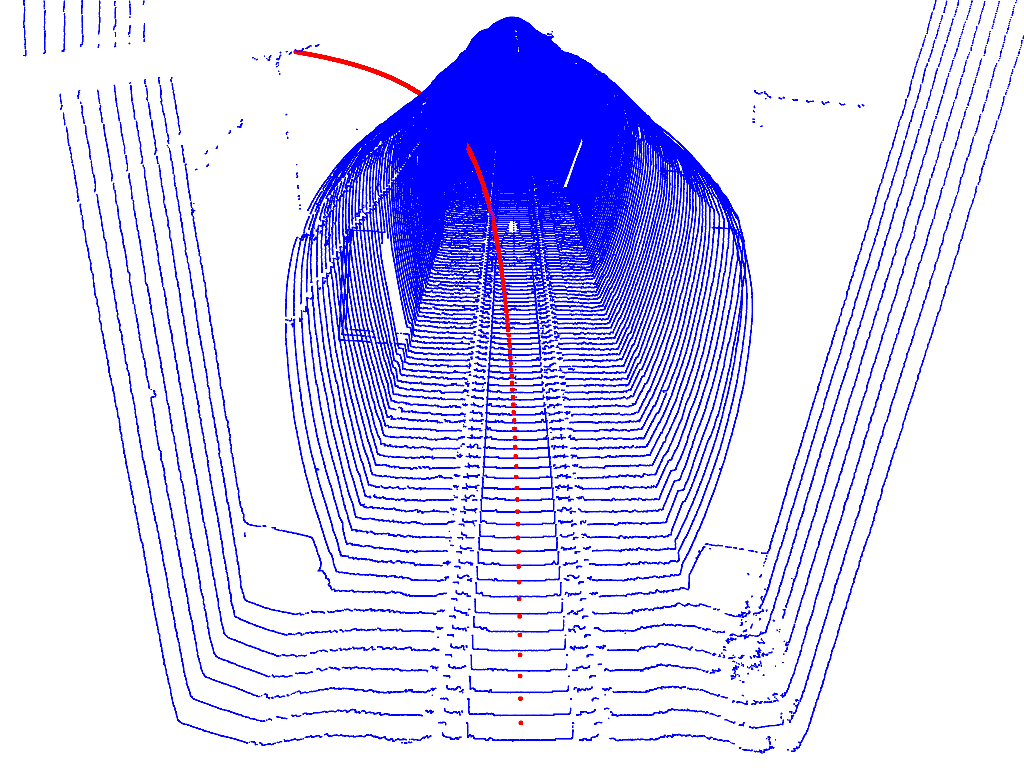
\includegraphics[height=3.2cm]{before_curving.png}\\
            {\scriptsize Pred transformacijo.}
        \end{column}
        \begin{column}{0.5\textwidth}
            \centering
            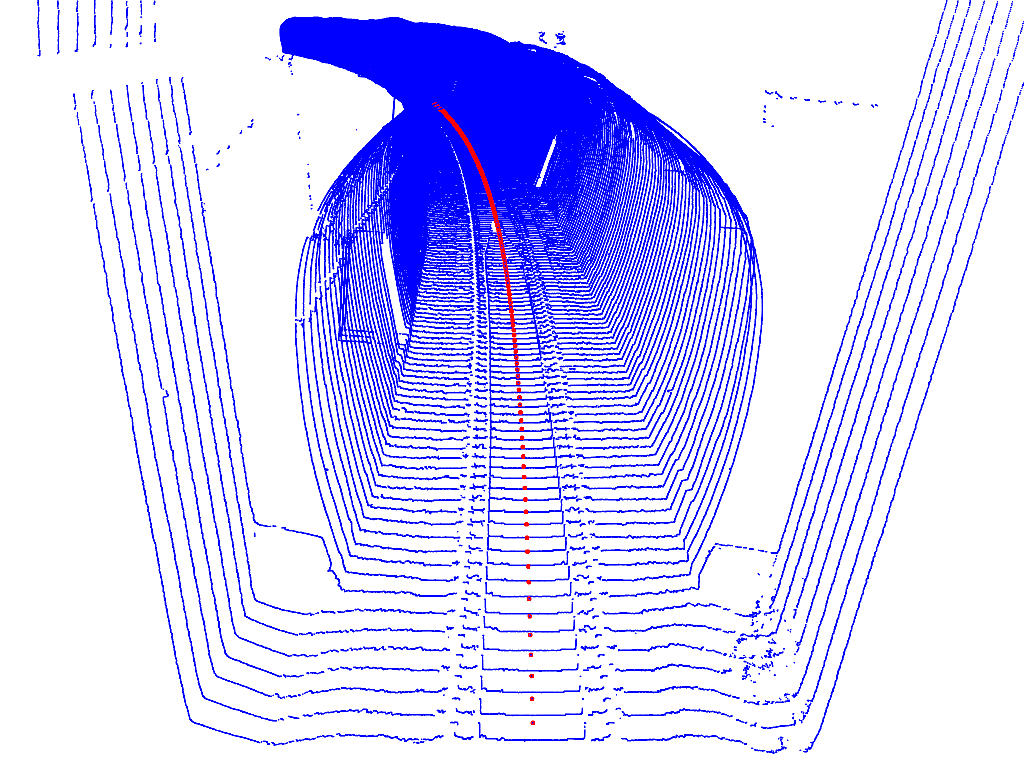
\includegraphics[height=3.2cm]{after_curving.png}\\
            {\scriptsize Po transformaciji.}
        \end{column}
    \end{columns}
\end{frame}

%----------------------------------------------------------------
% 5. B-zlepki
%----------------------------------------------------------------
\begin{frame}{Aproksimacija sten predora}
    \begin{columns}[T]
        \begin{column}{0.55\textwidth}
            \begin{itemize}
                \item Uporaba kubičnih B-zlepkov: tir/središčna linija \textbf{in} stene predora.
                \item Predor razdeljen na levo in desno polovico.
                \item L/D klasifikacija: vektorski produkt glede na tangento središčne linije.\\
                    {\scriptsize (primerjava koordinat ne deluje na ovinkih)}
            \end{itemize}
        \end{column}
        \begin{column}{0.45\textwidth}
            \centering
            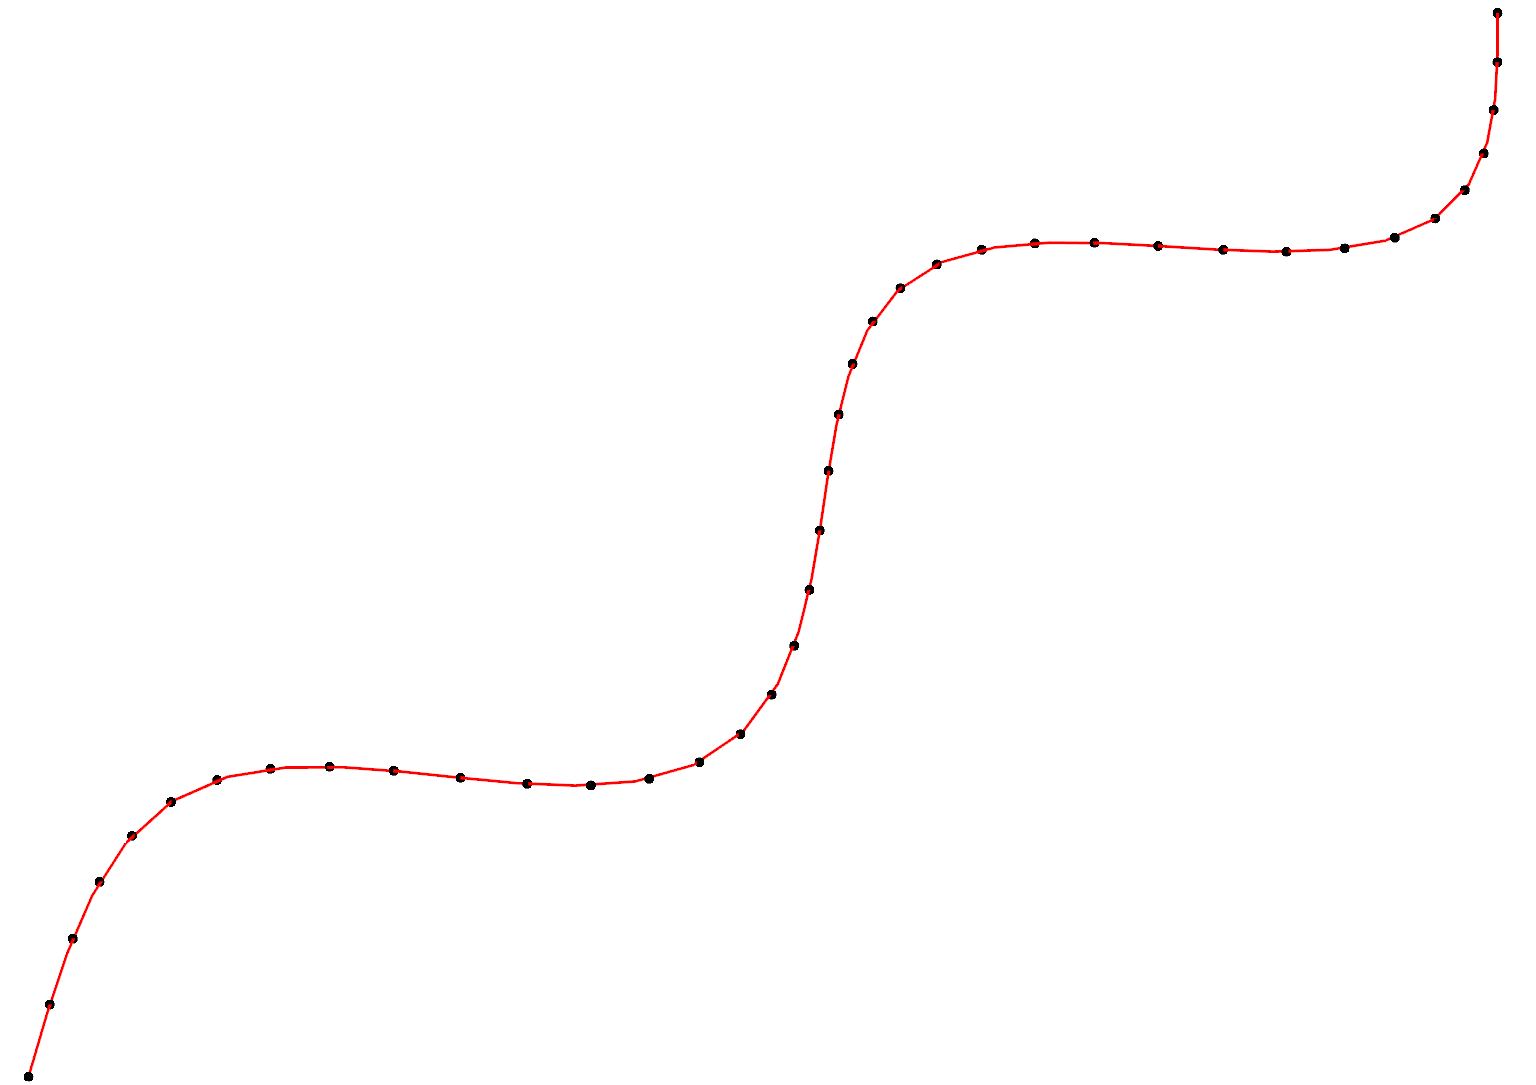
\includegraphics[height=4cm]{bspline.png}\\
            {\scriptsize Primer kubičnega B-zlepka.}
        \end{column}
    \end{columns}
\end{frame}
%----------------------------------------------------------------
% 6. Model vagona
%----------------------------------------------------------------
\begin{frame}{Geometrijski model vagona}
    \begin{columns}[T]
        \begin{column}{0.55\textwidth}
            \begin{itemize}
                \item Vagon: kvader.
                \item 2 osi: $\boldsymbol{p}_0$ (zadnja, na tiru), $\boldsymbol{p}_1$ (sprednja).
                \item $\boldsymbol{p}_1$: presečišče B-zlepka tira in kroga okrog $\boldsymbol{p}_0$ (polmer $=$ medosna razdalja).
                \item Sprednja os pravilno postavljena tudi v ovinkih.
                \item Izpeljava lokalnega koordinatnega sistema za pravilno premikanje kvadra.
            \end{itemize}
        \end{column}
        \begin{column}{0.45\textwidth}
            \centering
            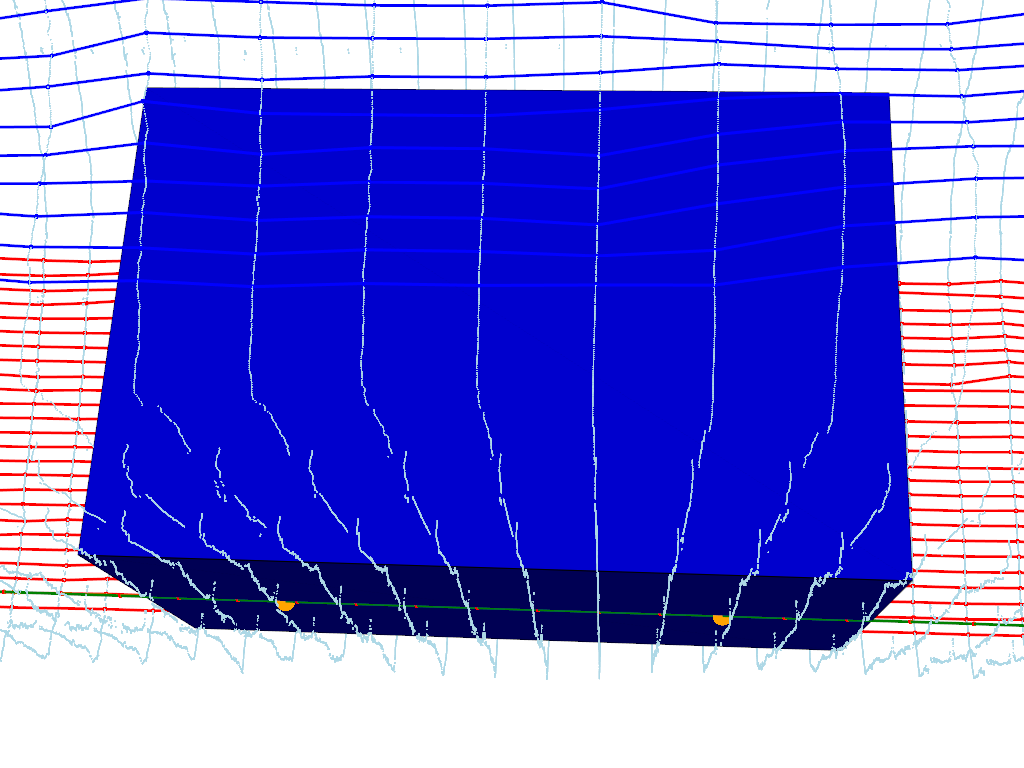
\includegraphics[width=\linewidth]{wheelbase.png}
        \end{column}
    \end{columns}
\end{frame}

%----------------------------------------------------------------
% 7. Kritične točke
%----------------------------------------------------------------
\begin{frame}{Kritične točke vagona}
    \begin{columns}[T]
        \begin{column}{0.5\textwidth}
            \begin{itemize}
                \item 6 kritičnih točk za vsako horizontalno plast.
                \item 3 vzdolžni položaji (zadaj, sredina, spredaj) $\times$ 2 strani (leva, desna).
            \end{itemize}
            \begin{equation*}
                \boldsymbol{c}_{s,p} = \boldsymbol{p}_{base,p} + s\cdot\tfrac{w}{2}\,\boldsymbol{r} + y\,\boldsymbol{u}
            \end{equation*}
            \centerline{\footnotesize \emph{za vsako vrednost $y$}}
            \begin{itemize}
                \item Pokrivajo robove, kjer je verjetnost trka največja.
                \item Višine $y$ so iste kot pri B-zlepkih sten, kar omogoča neposredno primerjavo z njimi.
            \end{itemize}
        \end{column}
        \begin{column}{0.5\textwidth}
            \centering
            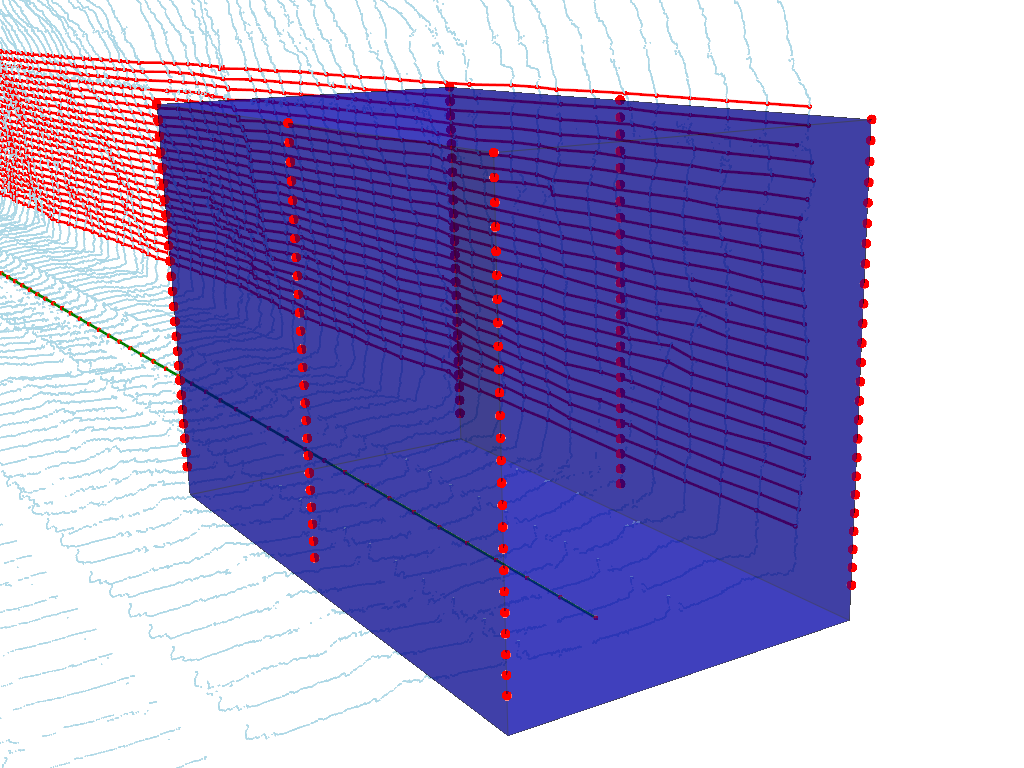
\includegraphics[width=\linewidth]{critical_points.png}
        \end{column}
    \end{columns}
\end{frame}


%================================================================
\section{Metodologija}
%================================================================

%----------------------------------------------------------------
% 8. Postopek zaznavanja trkov
%----------------------------------------------------------------
\begin{frame}{Postopek zaznavanja trkov}
    \begin{columns}[T]
        \begin{column}{0.55\textwidth}
            V vsakem koraku:
            \begin{itemize}
                \item posodobi položaj vagona,
                \item izračunaj 6 kritičnih točk $\forall y$.
            \end{itemize}

            \vspace{0.4em}
            Za vsako kritično točko:
            \begin{itemize}
                \item najdi najbližjo točko na B-zlepku stene,
                \item izračunaj razdaljo med njima,
                \item določi, ali je znotraj ali zunaj predora -- \\ vektorski produkt (kot za L/D).
            \end{itemize}
        \end{column}
        \begin{column}{0.45\textwidth}
            \centering
            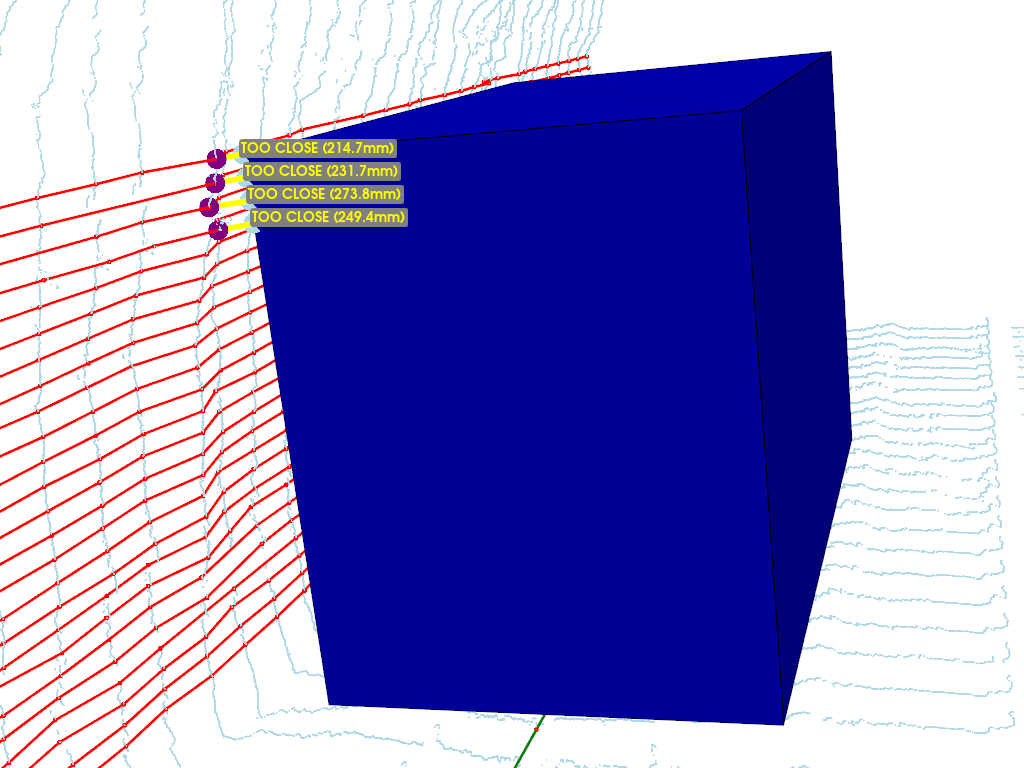
\includegraphics[width=\linewidth]{collision.png}
        \end{column}
    \end{columns}
\end{frame}

%----------------------------------------------------------------
% 9. Demonstracija simulacije
%----------------------------------------------------------------
\begin{frame}{Demonstracija simulacije}
    \begin{center}
        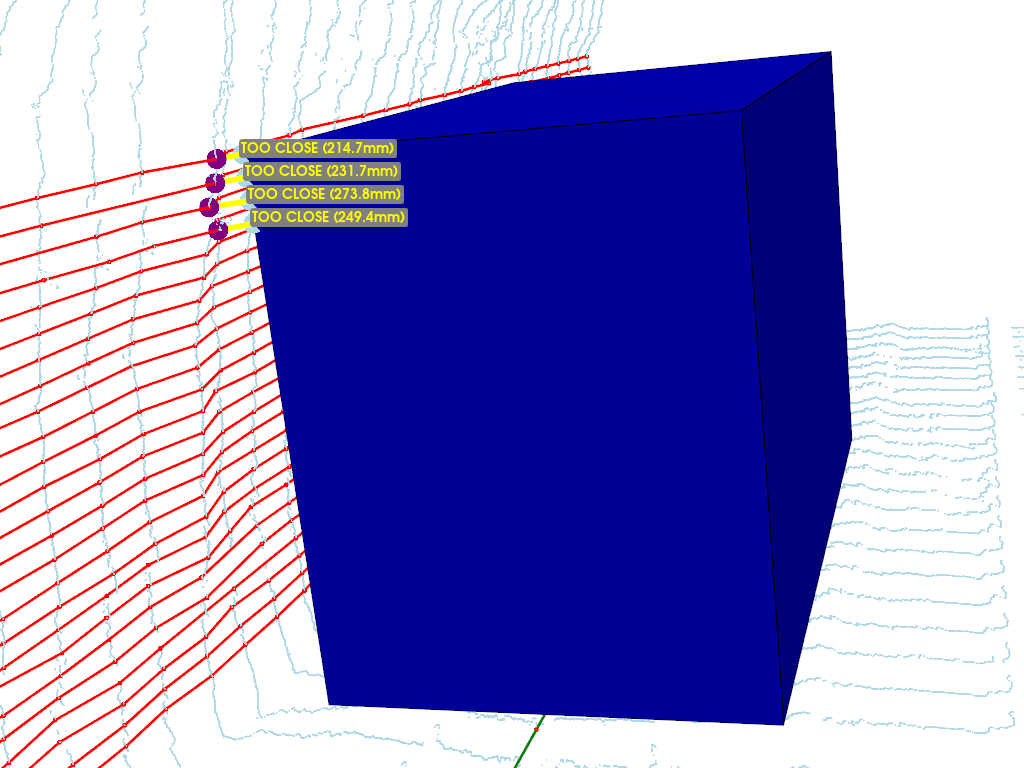
\includegraphics[height=6.5cm]{collision.png}
    \end{center}
\end{frame}

%----------------------------------------------------------------
% 10. Brušenje vagona
%----------------------------------------------------------------
\begin{frame}{Največji varni model vagona (brušenje)}
    \begin{columns}[T]
        \begin{column}{0.55\textwidth}
            \textbf{Cilj}: izpeljati največji vagon za dani predor.

            \vspace{0.3em}
            \textbf{Ideja}: prevelik vagon $\rightarrow$ \glqq{}obrusimo\grqq{} povsod, kjer zadene steno.

            \vspace{0.5em}
            \begin{itemize}
                \item Simulacija: povečan model, brez varnostne razdalje.
                \item Za vsak trk: zabeleži globino trka, zmanjšaj ustrezno dimenzijo.
                \item Rezultat: 3D model, ki izkorišča celoten profil predora.
            \end{itemize}
        \end{column}
        \begin{column}{0.45\textwidth}
            \centering
            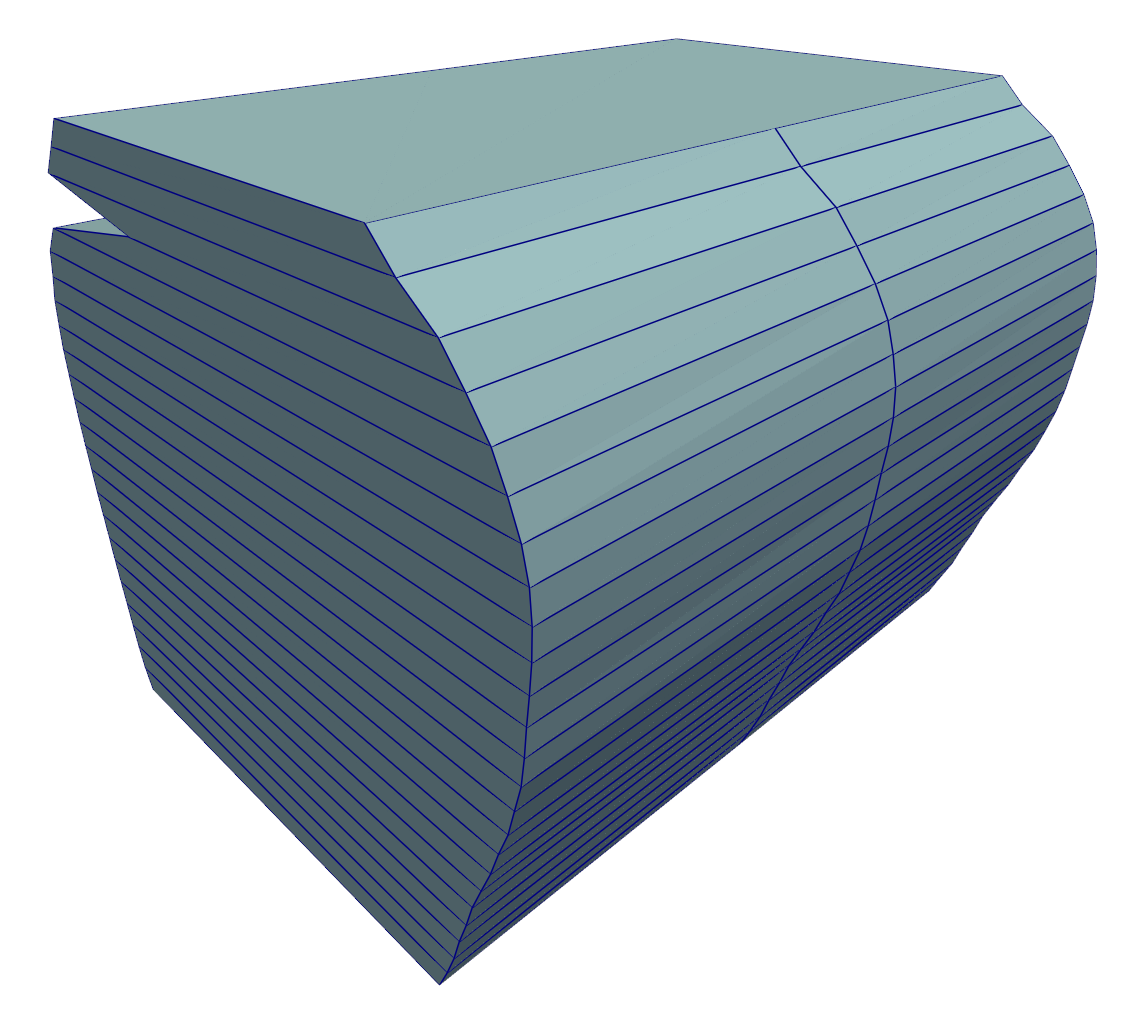
\includegraphics[width=\linewidth]{shaved_globoko.png}\\
            {\scriptsize Brušen model za predor Globoko.}
        \end{column}
    \end{columns}
\end{frame}

%----------------------------------------------------------------
% 11. Prileganje tovora
%----------------------------------------------------------------
\begin{frame}{Prileganje tovora}
    \begin{itemize}
        \item \textbf{Cilj}: poiskati rotacijo, pri kateri je tovor v celoti znotraj vagona.
    \end{itemize}

    \begin{algorithm}[H]
        \caption{Prileganje tovora v prilagojen model vagona}
        \begin{algorithmic}[1]
            \REQUIRE mreža tovora $\mathcal{C}$, model vagona $\mathcal{V}$, korak $\Delta = 45^{\circ}$
            \FOR{vsako kombinacijo orientacij (yaw, pitch, roll) s korakom $\Delta$}
                \STATE Obrni tovor $\mathcal{C}$ za kote (yaw, pitch, roll)
                \STATE Pretvori obrnjeni tovor v oblak točk $P$
                \IF{so vse točke $P$ vsebovane v $\mathcal{V}$}
                    \RETURN (yaw, pitch, roll)
                \ENDIF
            \ENDFOR
            \RETURN prileganje ni mogoče
        \end{algorithmic}
    \end{algorithm}
\end{frame}

%================================================================
\section{Eksperimentalno ovrednotenje}
%================================================================

%----------------------------------------------------------------
% 12. Testna predora
%----------------------------------------------------------------
\begin{frame}{Testna predora}
    \begin{columns}[T]
        \begin{column}{0.5\textwidth}
            \centering
            \textbf{Ringo} -- Trbovlje--Hrastnik\\
            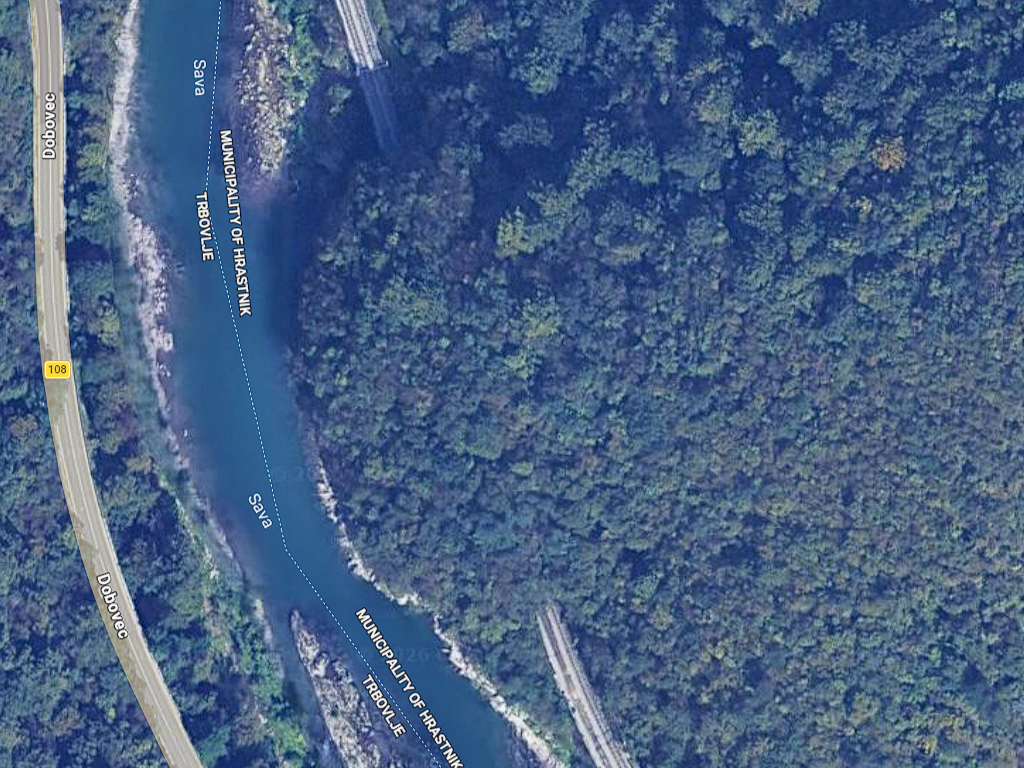
\includegraphics[height=2.4cm]{ringo_map.png}\hfill
            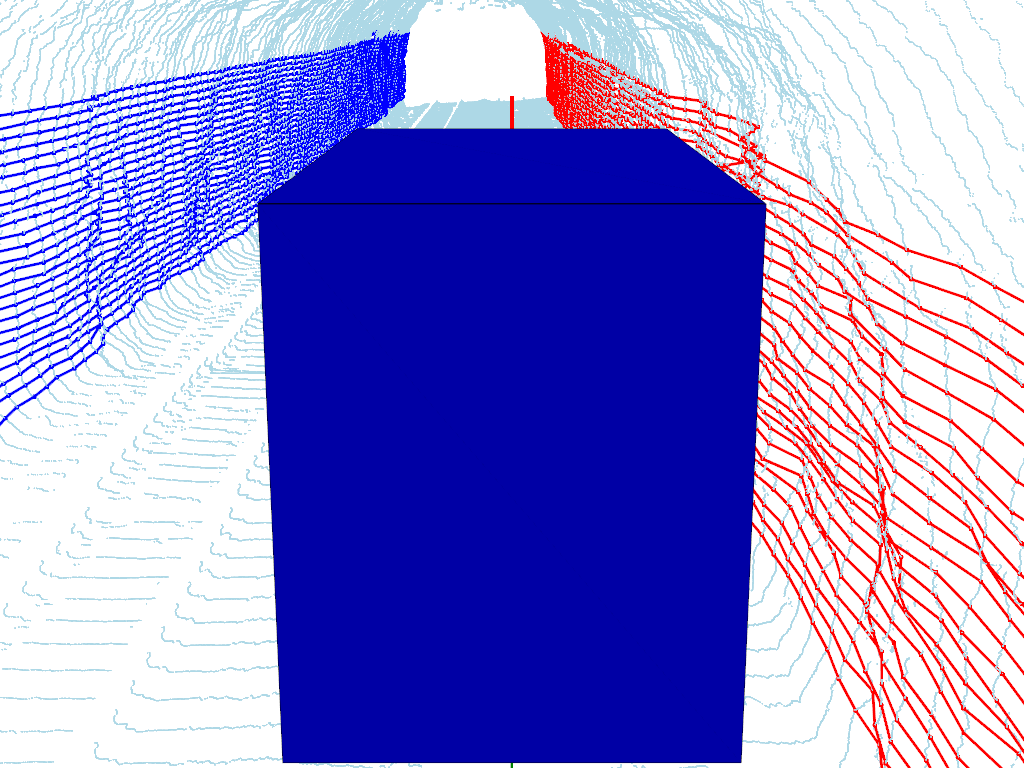
\includegraphics[height=2.4cm]{ringo.png}\\
            {\scriptsize 123 m, dvotirni, raven}
        \end{column}
        \begin{column}{0.5\textwidth}
            \centering
            \textbf{Globoko} -- Radovljica--Globoko\\
            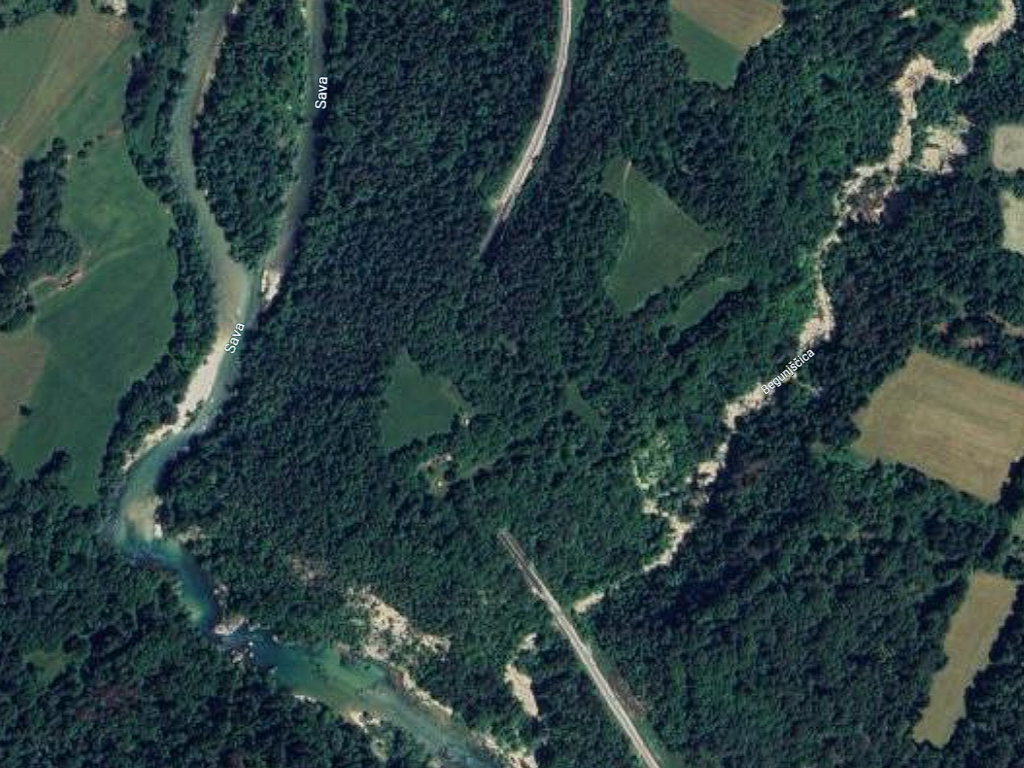
\includegraphics[height=2.4cm]{globoko_map.png}\hfill
            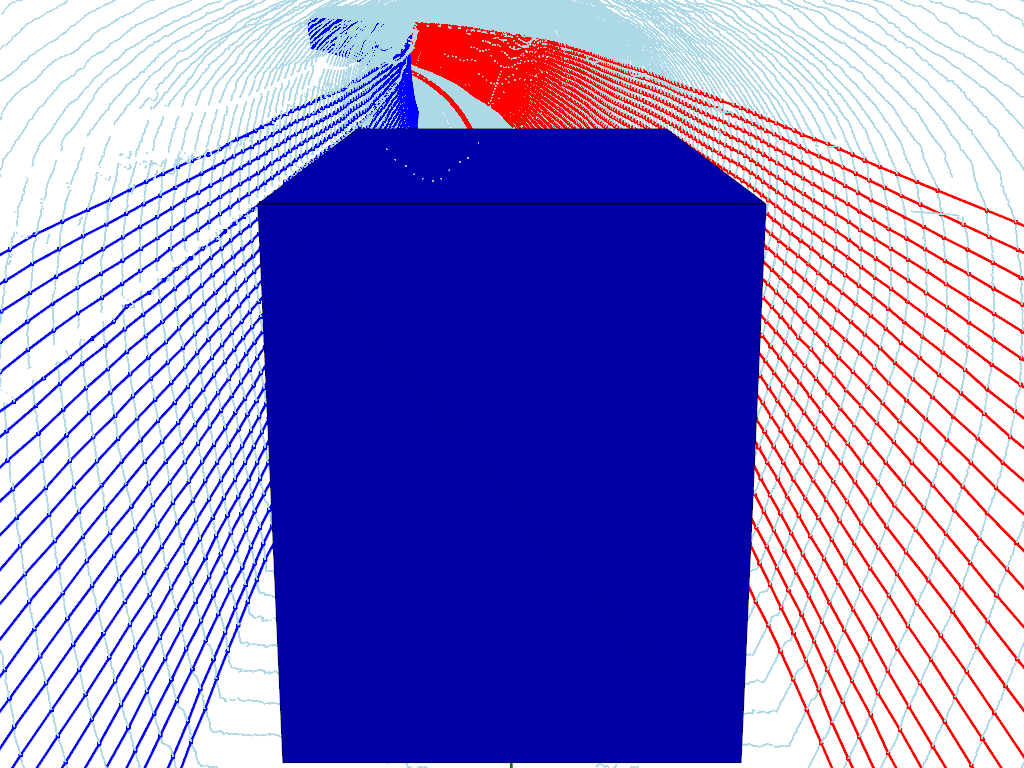
\includegraphics[height=2.4cm]{globoko.png}\\
            {\scriptsize 235 m, enotirni, ukrivljen}
        \end{column}
    \end{columns}

    \vspace{0.4em}
    \begin{center}
        \scriptsize
        \begin{tabular}{lrr}
            \toprule
            & \textbf{Ringo} & \textbf{Globoko} \\
            \midrule
            Število prečnih prerezov & 248 & 472 \\
            Velikost oblaka točk & 1.139.889 & 2.243.607 \\
            \bottomrule
        \end{tabular}
    \end{center}
\end{frame}

%----------------------------------------------------------------
% 13. Rezultati prileganja tovora
%----------------------------------------------------------------
\begin{frame}{Rezultati prileganja tovora}
    \begin{itemize}
        \item Po izpeljavi največjega varnega modela vagona $\Rightarrow$ prileganje tovorov.
        \item Tovora: enostavna zaboja (en na drugem) in tovor v obliki jadra.
    \end{itemize}

    \begin{columns}[T]
        \begin{column}{0.5\textwidth}
            \centering
            \textbf{Ringo}\\
            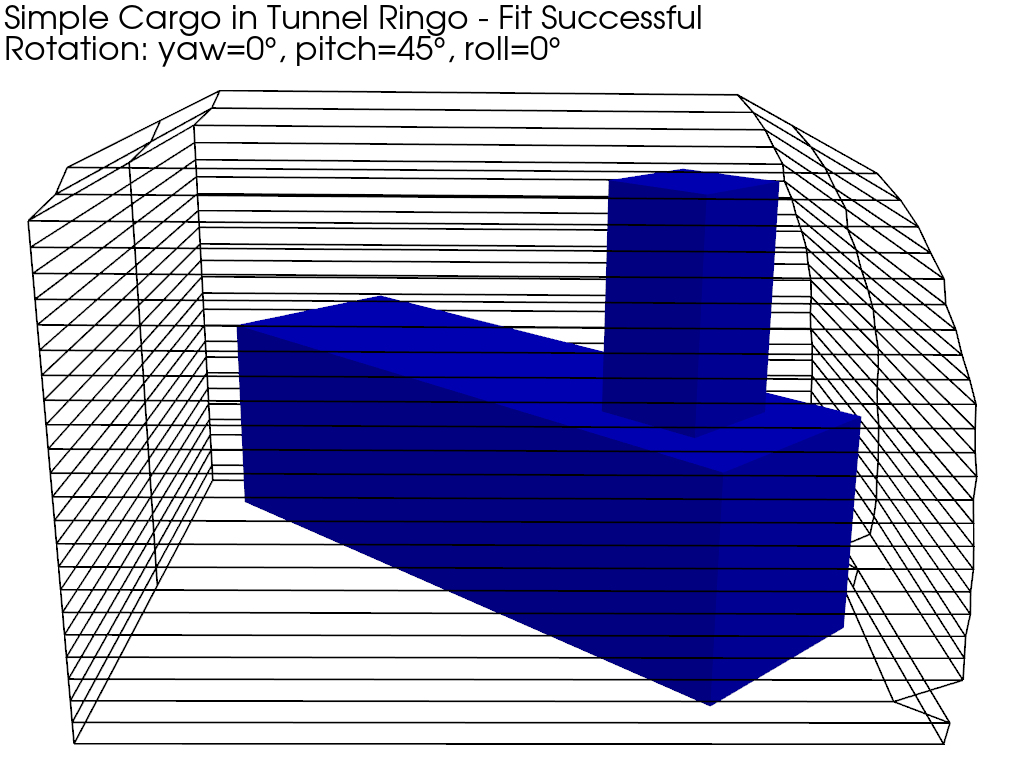
\includegraphics[height=2.8cm]{simple_ringo.png}\hfill
            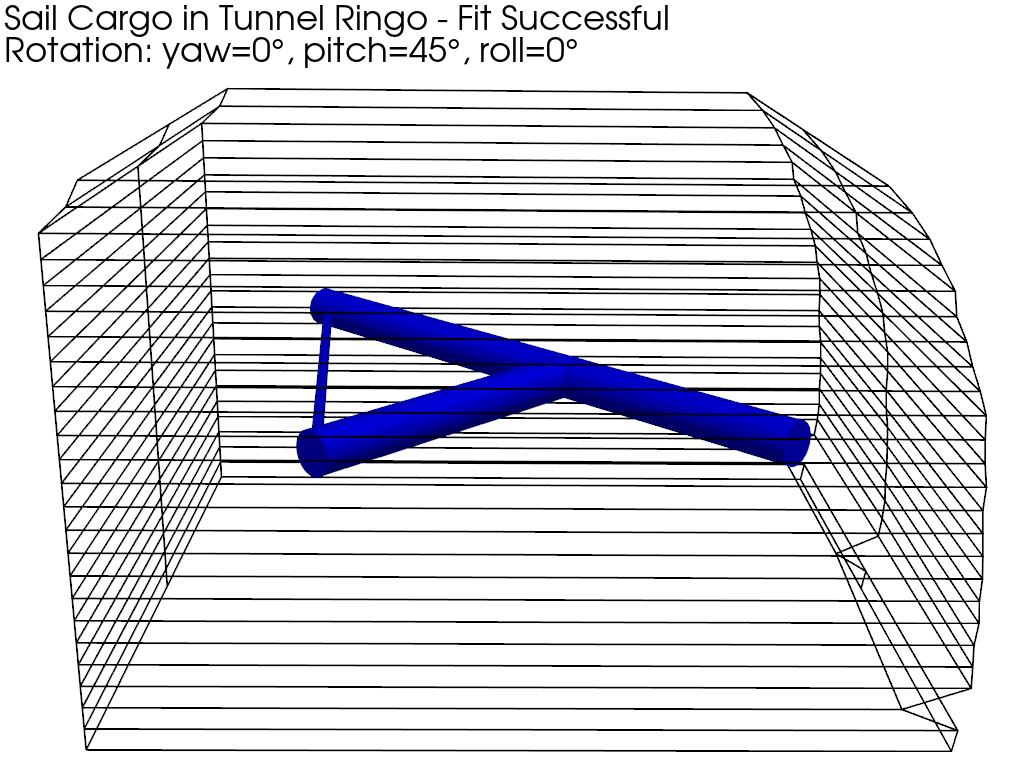
\includegraphics[height=2.8cm]{sail_ringo.png}\\
            {\scriptsize Oba uspešna pri kotu pitch $= 45^{\circ}$.}
        \end{column}
        \begin{column}{0.5\textwidth}
            \centering
            \textbf{Globoko}\\
            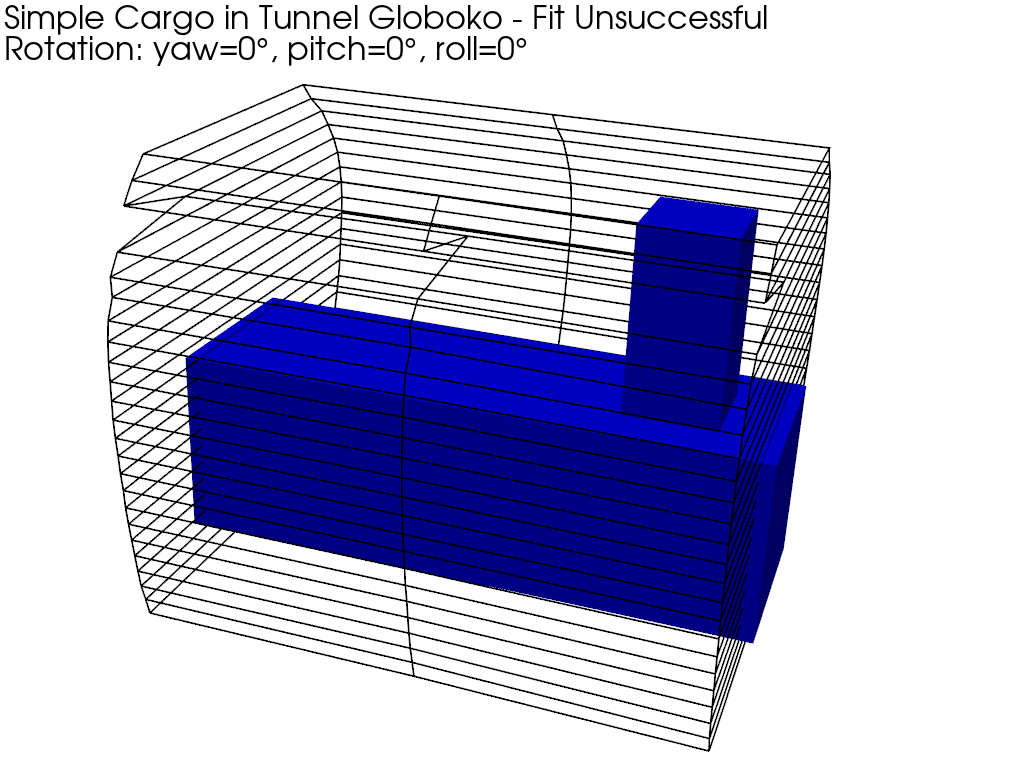
\includegraphics[height=2.8cm]{simple_globoko.png}\hfill
            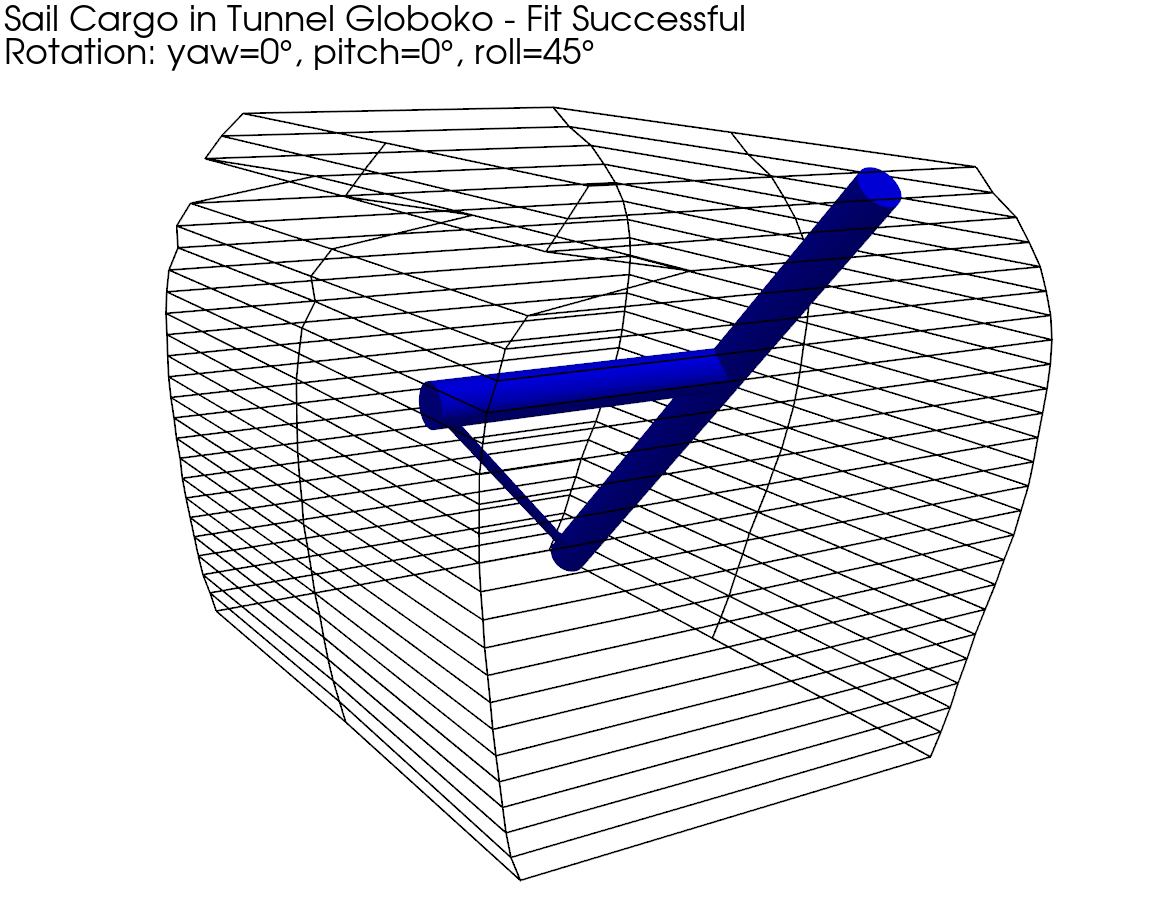
\includegraphics[height=2.8cm]{sail_globoko.png}\\
            {\scriptsize Zaboja se ne prilegata; jadro pri kotu roll $= 45^{\circ}$.}
        \end{column}
    \end{columns}

    \vspace{0.6em}
    \begin{itemize}
        \item Ožji profil predora $\Rightarrow$ manj izvedljivih orientacij in tovorov.
    \end{itemize}
\end{frame}

%----------------------------------------------------------------
% 14. Zmogljivost
%----------------------------------------------------------------
\begin{frame}{Analiza zmogljivosti}
    \begin{columns}[T]
        \begin{column}{0.55\textwidth}
            \scriptsize
            \begin{tabular}{lrrr}
                \toprule
                & $n$ & \textbf{Ringo [s]} & \textbf{Globoko [s]} \\
                \midrule
                Nalaganje & & 0{,}51 & 1{,}58 \\
                \midrule
                \multirow{4}{*}{Obdelava} & 10 & 1{,}10 & 3{,}17 \\
                & 25 & 2{,}66 & 7{,}39 \\
                & 50 & 4{,}90 & 14{,}57 \\
                & 200 & 19{,}81 & 59{,}00 \\
                \midrule
                Simulacija ($n=25$) & & 8{,}68 & 17{,}52 \\
                \bottomrule
            \end{tabular}
        \end{column}
        \begin{column}{0.45\textwidth}
            \begin{itemize}
                \item Trajanje $\sim$ linearno v $n$ in dolžini predora.
                \item Globoko (2$\times$ dolžina) $\Rightarrow$\\ $\sim$2$\times$ pri simulaciji,\\ $\sim$3$\times$ pri obdelavi.
            \end{itemize}
        \end{column}
    \end{columns}
\end{frame}

%================================================================
\section{Sklep}
%================================================================

%----------------------------------------------------------------
% 15. Sklep
%----------------------------------------------------------------
\begin{frame}{Sklepne ugotovitve}
    \textbf{Dosegli smo:}
    \begin{itemize}
        \item dinamično zaznavanje trkov v ukrivljenih predorih,
        \item največji varni model vagona za dani predor,
        \item prileganje tovora poljubnih oblik.
    \end{itemize}

    \textbf{Omejitve:} Kvaderski model, občutljivost na šum, 2 testna predora.

    \textbf{Naprej:}
    \begin{itemize}
        \item parametrični / CAD modeli vagonov,
        \item vzporedna obdelava z uporabo GPU,
        \item razširitev simulacije na celoten vlak.
    \end{itemize}
\end{frame}

%----------------------------------------------------------------
% 16. Hvala
%----------------------------------------------------------------
\begin{frame}{}
    \begin{center}
        {\Huge \textbf{Hvala za pozornost.}}
    \end{center}
\end{frame}

\end{document}
